\documentclass[conference]{IEEEtran}
\IEEEoverridecommandlockouts
% The preceding line is only needed to identify funding in the first footnote. If that is unneeded, please comment it out.
\usepackage{cite}
\usepackage{amsmath,amssymb,amsfonts}
\usepackage{algorithmic}
\usepackage{graphicx}
\usepackage{textcomp}
\usepackage{xcolor}

\usepackage[utf8]{vietnam}

\usepackage{amsthm}
% \usepackage{ntheorem}
\newtheoremstyle{theoremst}% name of the style to be used
  {\topsep}% measure of space to leave above the theorem. E.g.: 3pt
  {\topsep}% measure of space to leave below the theorem. E.g.: 3pt
  {\normalfont}% name of font to use in the body of the theorem
  {0pt}% measure of space to indent
  {\bfseries}% name of head font
  {.}% punctuation between head and body
  { }% space after theorem head; " " = normal interword space
  {\thmname{#1}\thmnumber{ #2}\textnormal{\thmnote{ (#3)}}}

\newtheoremstyle{examplest}% name of the style to be used
  {\topsep}% measure of space to leave above the theorem. E.g.: 3pt
  {\topsep}% measure of space to leave below the theorem. E.g.: 3pt
  {\normalfont}% name of font to use in the body of the theorem
  {0pt}% measure of space to indent
  {\bfseries}% name of head font
  {\\}% punctuation between head and body
  { }% space after theorem head; " " = normal interword space
  {\thmname{#1}\thmnumber{ #2}\textnormal{\thmnote{ (#3)}}}
  
\theoremstyle{theoremst}
\newtheorem{definition}{Định nghĩa}[section]
\newtheorem{theorem}{Định lý}[section]


\def\BibTeX{{\rm B\kern-.05em{\sc i\kern-.025em b}\kern-.08em
    T\kern-.1667em\lower.7ex\hbox{E}\kern-.125emX}}
\begin{document}


\title{MAGNN: Metapath Aggregated Graph Neural Network for
Heterogeneous Graph Embedding\\
{\footnotesize \textsuperscript{}Giảng viên hướng dẫn: TS. Đỗ Thị Thanh Hà}
\thanks{Identify applicable funding agency here. If none, delete this.}
}

\author{\IEEEauthorblockN{ Nguyễn Mạnh Linh}
% \IEEEauthorblockA{\textit{dept. name of organization (of Aff.)} \\
% \textit{name of organization (of Aff.)}\\
% City, Country \\
% email address or ORCID}
\and
\IEEEauthorblockN{Nguyễn Đức Thịnh}
% \IEEEauthorblockA{\textit{dept. name of organization (of Aff.)} \\
% \textit{name of organization (of Aff.)}\\
% City, Country \\
% email address or ORCID}
% \and
% \IEEEauthorblockN{3\textsuperscript{rd} Given Name Surname}
% \IEEEauthorblockA{\textit{dept. name of organization (of Aff.)} \\
% \textit{name of organization (of Aff.)}\\
% City, Country \\
% email address or ORCID}
% \and
% \IEEEauthorblockN{4\textsuperscript{th} Given Name Surname}
% \IEEEauthorblockA{\textit{dept. name of organization (of Aff.)} \\
% \textit{name of organization (of Aff.)}\\
% City, Country \\
% email address or ORCID}
% \and
% \IEEEauthorblockN{5\textsuperscript{th} Given Name Surname}
% \IEEEauthorblockA{\textit{dept. name of organization (of Aff.)} \\
% \textit{name of organization (of Aff.)}\\
% City, Country \\
% email address or ORCID}
% \and
% \IEEEauthorblockN{6\textsuperscript{th} Given Name Surname}
% \IEEEauthorblockA{\textit{dept. name of organization (of Aff.)} \\
% \textit{name of organization (of Aff.)}\\
% City, Country \\
% email address or ORCID}
}

\maketitle

\begin{abstract}
Một lượng lớn các đồ thị hay mạng trong thực tế vốn dĩ không đồng nhất, có nhiều loại nút và nhiều loại quan hệ. Embedding đồ thị không đồng nhất là việc embed từ cấu trúc lớn và nhiều thông tin của đồ thị về biểu diễn nút trong không gian thấp chiều. Các mô hình đã tồn tại tường định nghĩa metapaths trong một đồ thị không đầu nhất để ghi lại các quan hệ và định hướng lựa chọn "hàng xóm". Tuy nhiên các mô hình này bỏ qua đặc trưng của từng nút mà tìm hiểu ngay lập tức các nút trên metapath hoặc chỉ xem xét một metapath. Để khắc phục ba giới hạn này, tác giả đề xuất một mô hình mới là \textit{Metapath Aggregated
Graph Neural Network} (MAGNN) để tăng tốc hiệu năng cuối cùng. Đặc biệt, MAGNN sử dụng ba thành phần chính, biến đổi nội dung của nút thành các thuộc tính đóng gói của nút đầu vào, tổng hợp intra-metapath để kết hợp các nút ngữ nghĩa trung gian và tổng hợp inter-metapath để kết hợp thông tin từ nhiều metapaths. Các thí nghiệm được thực hiện trên ba bộ dữ liệu đồ thị không đồng nhất trong thực tế để phân loại nút, phân cụm nút và dự đoán liên kết chỉ ra rằng MAGNN đạt được kết quả dự đoán chính xác hơn so với các mô hình state-of-the-art hiện tại .
\end{abstract}

% \begin{IEEEkeywords}
% component, formatting, style, styling, insert
% \end{IEEEkeywords}

\section{Giới thiệu}
Nhiều bộ dữ liệu thực tế được biểu diễn với cấu trúc dữ liệu đồ thị, trong đó các đối tượng và quan hệ giữa chúng được biểu diễn bằng các nút và cạnh. Các ví dụ bao gồm mạng xã hội [14, 29], hệ thống vật lý [2, 10], mạng giao thông [18, 34], mạng trích dẫn [1, 14, 16], hệ thống gợi ý [26, 35], đồ thị tri thức [3, 24], ... Bản chất non-Euclidean của đồ thị khiến chúng khó được mô hình hóa bằng các mô hình học máy truyền thống. Với tập lân cận của mỗi nút, không hề có thứ tự hoặc giới hạn về kích thước, Tuy nhiên, hầu hết các mô hình thống kê giả định rằng một đầu vào có thứ tự và kích thước cố định trong không gian Euclid. Do đó, sẽ thuận tiện nếu các nút có thể được biểu diễn bằng các vector thấp chiều trong không gian Euclid và từ đó có thể lấy làm đầu vào của mô hình học máy khác. 

Các kĩ thuật embed đồ thị khác nhau được đề xuất cho cấu trúc dữ liệu đồ thị. LINE [25] sinh node embedding dựa vào các nút gần nhất và gần thứ 2. Các phương pháp dựa trên bước ngẫu nhiên (Random-walk) bao gồm DeepWalk [21], node2vec [13] và TADW [32] sinh dãy nút được sinh ra bởi các bước ngẫu nhiên đến một mô hình skip-gram [19] để học node embeddings. Với sự phát triển nhanh chóng của deep learning, mạng neuron đồ thị (Graph neural networks - GNNs) được đề xuất, mô hình học các biểu diễn đồ thị bằng việc sử dụng các lớp neuron được thiết kế đặc biệt. Spectral-based GNNs bao gồm ChebNet [8] và GCN [16] biểu diễn các toán tử tích chập đồ thị trong miền Fourier của một đồ thị đầy đủ. Các mô hình dựa trên spatial, bao gồm GraphSAGE [14], GAT [28] và nhiều biến thể khác [17, 34, 45], giải quyết các vấn đề xung quanh khả năng mở rộng và khả năng tổng quát hóa của các mô hình dựa trên phổ bằng cách biểu diễn các phép toán tích chập đồ thị trực tiếp trên miền đồ thị. 

Mặc dù GNNs đã đạt được những kết quả tốt nhất trong nhiều bài toán, hầu hết các mô hình dựa trên GNN giả định rằng đầu vào là đồ thị đồng nhất với chỉ một loại nút và một loại cạnh. Hầu hết đồ thị trong thực tế bao gồm nhiều loại nút và cạnh tương ứng với các thuộc tính trong các không gian thuộc tính khác nhau. Ví dụ, một mạng đồng tác giả chứa ít nhất hai loại nút, cụ thể là các tác giả và bài báo. Các thuộc tính của tác giả có thể bao gồm nơi làm việc, trích dẫn và lĩnh vực nghiên cứu. Thuộc tính của bài báo bao gồm từ khóa, địa điểm, năm phát hành ... Tác giả gọi loại đồ thị này là \textit{mạng thông tin không đồng nhất} (HINs) hoặc \textit{đồ thị không đồng nhất.}
 Sự không đồng nhất trong cả cấu trúc biểu diễn và nội dung của nút khiến GNN gặp khó khăn trong việc mã hóa thông tin vào không gian vector thấp chiều. 

 Hầu hết các phương pháp nhúng đồ thị không đồng nhất hiện có dựa trên ý tưởng về metapaths. Một \textit{metapath} là một trình tự có thứ tự của các loại nút và loại cạnh được xác định trên lược đồ mạng, mô tả mối quan hệ tổng hợp giữa các loại nút liên quan. Ví dụ một mạng với tác giả, bài báo và dịa điểm, \textit{Tác giả-Bài báo-Tác giả} (APA) và \textit{Tác giả-Bài báo-Địa điểm-Bài báo-Tác giả} (APVPA) là các metapaths mô tả mối quan hệ khác nhau giữa các tác giả. Metapath APA tương ứng với hai đồng tác giả, trong khi APVPA tương ứng với hai tác giả xuất bản bài báo cùng địa điểm. Do đó, ta có thể xem metapath là khoảng cách gần bậc cao giữa 2 nút. Do GNNs truyền thống xử lý tất cả các nút như nhau, chúng không thể mô hình hóa cấu trúc phức tạp và thông tin có nghĩa trong đồ thị không đồng nhất.


 Mặc dù các phương pháp nhúng dựa trên metapath này hoạt động tốt hơn phương pháp nhúng mạng truyền thống trên các bài toán khác nhau, chẳng hạn như phân loại nút và dự đoán liên kết, chúng vẫn có ít nhất một trong những hạn chế sau. (1) Mô hình không sử dụng đặc trưng về nội dung nút nên nó hiếm khi hoạt động tốt với các đồ thị không đồng nhất với nút có nội dung nhiều đặc trưng (ví dụ metapath2vec [9], ESim [22], HIN2vec [11], HERec [23]). (2) Mô hình loại bỏ tất cả các nút trên metapath, chỉ xem xét 2 nút cuối dẫn đến mất thông tin (ví dụ HERec [23] and HAN [31]). (3) Mô hình dựa trên một metapath duy nhất để nhúng đồ thị không đồng nhất. Do đó, mô hình yêu cầu một quá trình chọn metapath thủ công và mất đi các đặc điểm của thông tin từ các metapaths khác dẫn đến hiệu năng không tối ưu (ví dụ metapath2vec [9]). 

 Để giải quyết các hạn chế này, tác giả đề xuất một mạng neuron tổng hợp metapath (\textit{Metapath Aggregated Graph Neural Network - MAGNN}) mới cho việc nhúng đồ thị không đồng nhất. MAGNN giải quyết tất cả các vấn đề được mô tả ở trên bằng cách áp dụng chuyển đổi nội dung nút, tổng hợp nội intra-metapath và tổng hợp inter-metapath để tạo nút nhúng. Cụ thể, MAGNN trước tiên áp dụng biến đổi tuyến tính theo loại cụ thể để chiếu các thuộc tính nút không đồng nhất với số chiều có thể không bằng nhau cho các loại nút khác nhau, cho cùng một không gian latent. Tiếp theo, MAGNN áp dụng intra-metapath với cơ chế chú ý [28] cho mọi metapath. Trong tổng hợp intra-metapath này, mỗi nút đích trích xuất và kết hợp thông tin từ các cấu hình metapath kết nối với nút lân cận dựa trên metapath của nó. Bằng cách này, MAGNN nắm bắt được thông tin về cấu trúc và ngữ nghĩa của các đồ thị không đồng nhất từ cả các nút lân cận và bối cảnh metapath giữa chúng. Sau khi tổng hợp intra-metapath, MAGNN tiếp tục tiến hành tổng hợp inter-metapath bằng cách sử dụng cơ chế chú ý để hợp nhất các latent vector thu được từ nhiều metapaths vào các nút nhúng cuối cùng. Bằng cách tích hợp nhiều metapaths, mô hình của tác giả có thể học ngữ nghĩa toàn diện ẩn giấu trong đồ thị không đồng nhất. 

Tóm lại, bài báo này có một số đóng góp chính:
\begin{itemize}
  \item[] (1) Tác giả đề xuất một mạng neuron đồ thị mới  dựa trên tổng hợp metapath để nhúng nhúng đồ thị không đồng nhất.
  \item[] (2) Thiết kế một số hàm mã hóa tiềm năng để trích xuất thông tin từ các cấu hình metapaths, bao gồm trường hợp dựa trên ý tưởng phép xoay quan hệ trong không gian phức [24].
  \item[] (3) Tác giả tiến hành nhiều thí nghiệm trên các tập dữ liệu IMDb và DBLP để phân loại và phân cụm nút cũng như dùng tập Last.fm để đánh giá dự đoán liên kết và hiệu suất của mô hình. Thí nghiệm trên tất cả các tập dữ liệu này và các bài toán chỉ ra rằng nhúng nút được học bởi MAGNN luôn tốt hơn các mô hình tiên tiến nhất hiện tại (SOTA).
\end{itemize}


\section{Sơ lược}
Trong phần này, tác giả đưa ra các định nghĩa chuẩn của một số thuật ngữ quan trọng liên quan đến đồ thị không thuần nhất. Minh họa trong hình 1. Bên cạnh đó bảng 1 tóm tắt các kí hiệu được sử dụng nhiều trong báo cáo để thuận tiện cho việc tra cứu nhanh.

\begin{definition}
\textbf{Đồ thị không đồng nhất.} Một đồ thị không đồng nhất được định nghĩa là một đồ thị $\pmb{\mathcal{G}} = (\pmb{\mathcal{V}}, \pmb{\mathcal{E}})$ với ánh của loại nút $\phi: \pmb{\mathcal{V}} \to \pmb{\mathcal{A}}$ và ánh xạ của loại cạnh $\psi: \pmb{\mathcal{E}} \to \pmb{\mathcal{R}}$. $\pmb{\mathcal{A}}$ và $\pmb{\mathcal{R}}$ lần lượt là các tập loại nút và loại cạnh với $|\pmb{\mathcal{A}}| + |\pmb{\mathcal{R}}| > 2$.
\end{definition}

\begin{definition}
  \textbf{Metapath.} Một metapath $P$ được định nghĩa là một đường đi lập thành từ $A_1  \xrightarrow{R_1} A_2  \xrightarrow{R_2} ... \xrightarrow{R_l} A_{l+1}$ (viết tắt là $A_1 A_2 ... A_{l+1}$) mô tả một quan hệ tổng hợp $R = R_1 \circ R_2 \circ ... \circ R_l$ giữa các loại nút $A_1$ và $A_{l+1}$, trong đó $\circ$ là toán tử tổng hợp trên các quan hệ.
\end{definition}

\begin{definition}
  \textbf{Cấu hình metapath.} Cho một metapath $P$ của một đồ thị không đồng nhất, một cấu hình metapath $p$ của $P$ được định nghĩa là một dãy các nút trong đồ thị theo lược đồ được xác định bởi $P$.
\end{definition}

\begin{definition}
  \textbf{Lân cận dựa trên metaptah.} Cho một metapath $P$ của một đồ thị không đồng nhất, các lân cận dựa trên metapath $\pmb{\mathcal{N}}_\upsilon ^ P$ của một nút $\upsilon$ được định nghĩa là tập hợp các nút liên kết với nút $\upsilon$ qua các cấu hình metapath của $P$. Một lân cận được kết nối bởi hai cấu hình metapath khác nhau được đánh giá như hai nút khác nhau trong $\pmb{\mathcal{N}}_\upsilon ^ P$. Lưu ý rằng $\pmb{\mathcal{N}}_\upsilon ^ P$ bao gồm chính nút $\upsilon$ nếu $P$ đối xứng.

  Ví dụ, xem xét tập dữ liệu UATA trong hình 1, nghệ sĩ \textit{Queen} là một lân cân dựa trên metapath của người dùng \textit{Bob}. Hai nút này được kết nối thông qua cấu hình metapath \textit{Bob-Beatles-Rock-Queen}. Hơn nữa, chúng ta có thể tham chiếu tới \textit{Beatles} và \textit{Rock} như là các nút trung gian trên cấu hình metapath này.
\end{definition}

\begin{definition}
  \textbf{Đồ thị dựa trên metapath.} Cho một metapath $P$ của một đồ thị không đồng nhất $\pmb{\mathcal{G}}$, đồ thị dựa trên metapath $\pmb{\mathcal{G}}^P$ là một đồ thị được xây dựng bởi tất cả các cặp lân cận dựa trên metapath $P$ trong đồ thị $\pmb{\mathcal{G}}$. Lưu ý rằng $\pmb{\mathcal{G}}^P$ là đồng nhất nếu $P$ đối xứng.
\end{definition}

\begin{definition}
  \textbf{Biểu diễn đồ thị không đồng nhất.} Cho một đồ thị không đồng nhất $\pmb{\mathcal{G}} = (\pmb{\mathcal{V}}, \pmb{\mathcal{E}})$ với các ma trận thuộc tính nút $\pmb{X}_{A_i} \in \mathbb{R} ^ {|\pmb{\mathcal{V}}_{A_i}| \times d_{A_i}}$ của các loại nút $A_i \in \pmb{\mathcal{A}}$, biểu diễn đồ thị không đồng nhất là việc học các biểu diễn nút $d$ chiều $\pmb{h}_{\upsilon} \in \mathbb{R}^d$ với mọi $\upsilon \in \pmb{\mathcal{V}}$ với $d \ll |\pmb{\mathcal{V}}|$ có thể ghi lại thông tin cấu trúc và ngữ nghĩa liên quan đến $\pmb{\mathcal{G}}$.
\end{definition}

\begin{figure*}
  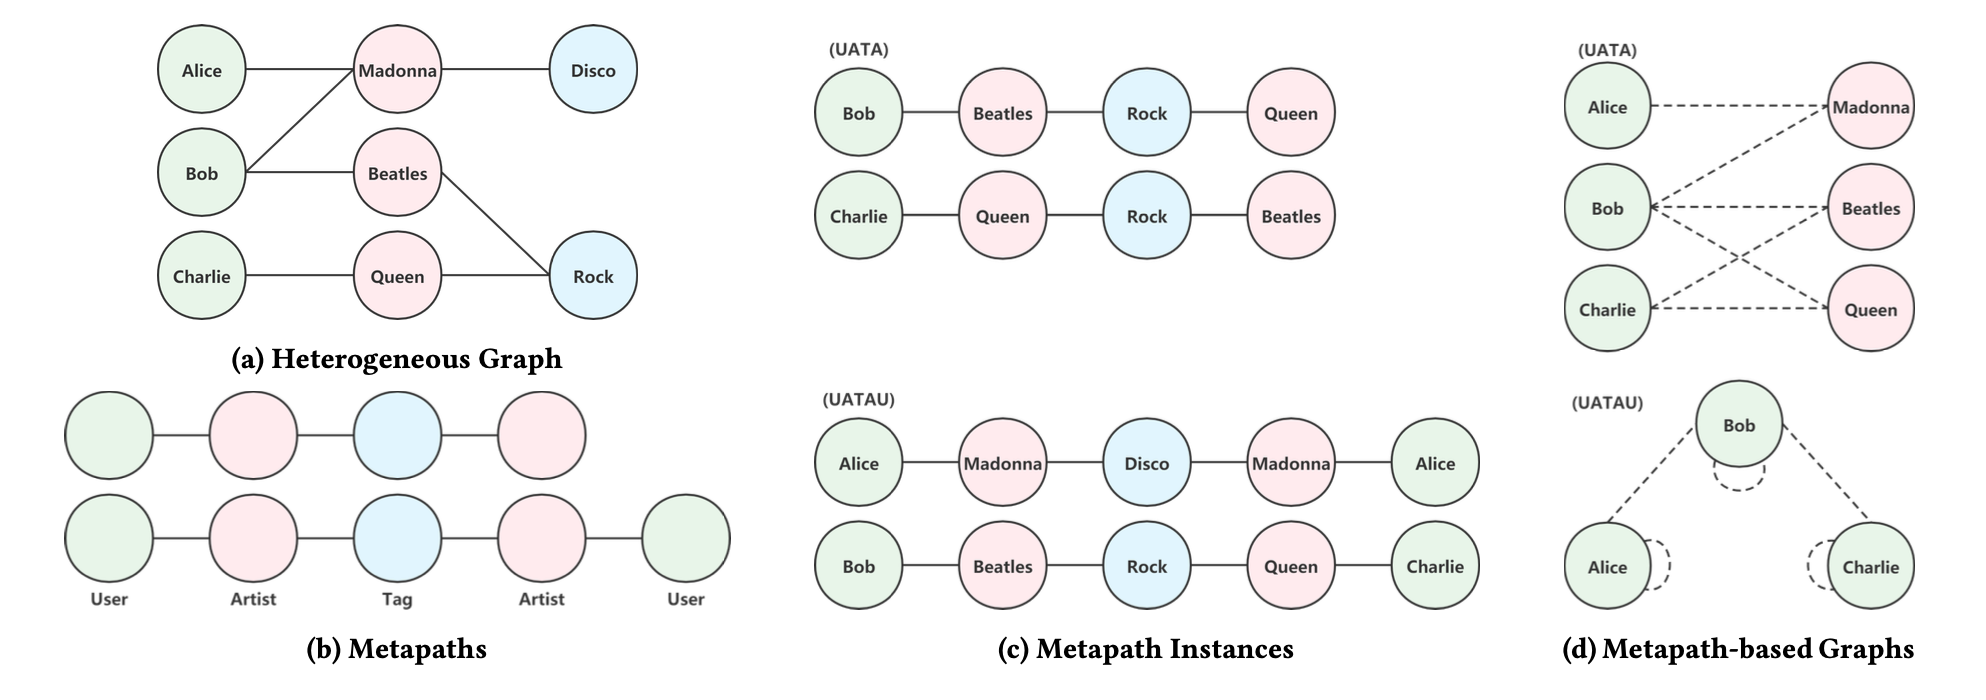
\includegraphics[width=\textwidth]{figs/fig1.png}
  \caption{Minh họa các thuật ngữ được định nghĩa trong Phần 2. (a) Một ví dụ về đồ thị không đồng nhất với ba loại nút (người dùng, nghệ sĩ, thẻ). (b) metapath Người dùng-Nghệ sĩ-Thẻ-Nghệ sĩ (UATA) và metapath Người dùng-Nghệ sĩ-Thẻ-Nghệ sĩ-Người dùng (UATAU). (c) Ví dụ các cấu hình metapath của UATA, UATAU. (d) Đồ thị dựa trên metapath cho UATA và UATAU.}
\end{figure*}





\section{Nghiên cứu liên quan}
Trong phần này, tác giả xem lại các nghiên cứu về học biểu diễn đồ thị liên quan tới mô hình của tác giả. Chúng được chia thành hai phần nhỏ: phần đầu tóm tắt các nỗ lực nghiên cứu về GNN cho việc nhúng đồ thị, phần sau giới thiệu các phương pháp nhúng đồ thị cho các đồ thị không đông nhất.

\subsection{Mạng neuron đồ thị}
Mục tiêu của một GNN là học một biểu diễn vector thấp chiều $\pmb{h}_{\upsilon}$ cho mọi nút $\upsilon$, cách được sử dụng cho nhiều tác vụ downstream, ví dụ như phân loại nút, phân cụm nút và dự đoán liên kết. Lý do đằng sau điều này là mỗi nút được xác định một cách tự nhiên bởi các đặc trưng và khu vực lân cận của nó. Theo ý tưởng này và dựa trên quá trình xử lý tín hiệu đồ thị, GNNs dựa trên phổ được phát triển để thực hiện tích chập đồ thị trong miền Fourier của một đồ thị. ChebNet [8] sử dụng các đa thức Chebusev để lọc các tín hiệu đồ thị (đặc trưng nút) trong miền Fourier của đồ thị. Một mô hình có ảnh hưởng khác thuộc loại này là GCN [16], nó ràng buộc và đơn giản hóa các tham số của ChebNet để giảm bớt vấn đề overfitting và cải thiện hiệu năng. Tuy nhiên, GNNs dựa trên phổ có khả năng mở rộng và tổng quát kém vì chúng yêu cầu toàn bộ đồ thị làm đầu vào cho mọi lớp và các bộ lọc đã được học của chúng phụ thuộc vào cơ sở riêng của Laplacian của đồ thị, liên quan chặt chẽ đến cấu trúc đồ thị cụ thể.

GNNs dựa trên spatial đã được đề xuất để khắc phục những giới hạn này. GNNs kiểu này định nghĩa các tích chập một cách trực tiếp trong miền đồ thị bằng cách tổng hợp thông tin từ các lân cận của mỗi nút, giống như các toán tử tích chập trong mạng tích chập xử lý dữ liệu hình ảnh. GraphSAGE [14], một framework GNN dựa trên spatial được tạo ra dựa trên khái niệm chung về các hàm tổng hợp để tạo các nút nhúng hiệu quả. Các mẫu hàm tổng hợp và biến đổi một lân cận của nút mục tiêu và do đó tạo điều kiện huấn luyện song song và tổng quát hóa cho các nút hoặc đồ thị ẩn. Rất nhiều biến thể của GNN dựa trên spatial được đề xuất dựa trên ý tưởng này. Lấy cảm ứng từ Transformer [27], GAT [28] kết hợp cơ chế chú ý vào hàm tổng hợp để đưa vào độ quan trọng tương đối của thông tin của mỗ lân cận từ góc nhìn của nút đích. GGNN [17] thêm một thành phần lặp có kiểm soát (GRU) [7] vào hàm tổng hợp bằng cách xử lý thông tin vùng lân cận được tổng hợp làm đầu vào cho GRU của bước thời gian hiện tại. GaAN [34] kết hợp GRU với cơ chế chú ý nhiều đầu để  thỏa mãn không thời gian đồ thị. STAR-GCN [35] dử dụng nhiều bộ mã hóa-giải mã GCN để
tăng hiệu suất dự đoán xếp hạng. 

Tất cả các GNN được đề cập ở trên đều được xây dựng cho các đồ thị đồng nhất hoặc được thiết kế cho một số đồ thị với cấu trúc đặc biệt như là trong các hệ thống gợi ý người dùng - sản phẩm. Do hầu hết các GNNs hiện tại hoạt động trên đặc trưng của các nút trong cùng không gian nhúng được chia sẻ, chúng không thể đáp ứng một cách tự nhiên với các đồ thị không đồng nhất với các đặc trung nút nằm trên các không gian khác nhau.

\subsection[short]{Nhúng đồ thị không đồng nhất}
Nhúng đồ thị không đồng nhất nhằm mục đích chiếu các nút từ một đồ thị không đồng nhất vào một không gian vector thấp chiều. Chủ đề thách thức này thu hút rất nhiều nghiên cứu. Ví dụ, metapath2vec [9] sinh các bước ngẫu nhiên được hướng dẫn bởi một meta-path đơn, thứ sau đó được lấy làm đầu vào cho mô hình skip-gram [19] để sinh các nút nhúng. Với metapaths được định nghĩa trước, ESim [22] sinh các nút nhúng bằng cách học từ các cấu hình metapath mẫu âm và dương. HIN2vec [11] thực hiện nhiều tác vụ huấn luyện để học các biểu diễn của nút và metapaths của một đồ thị không đồng nhất. Cho một metapath, HERec [23] chuyển đổi một đồ thị không đồng nhất thành một đồ thị đồng nhất dựa trên các lân cận metapath-based và áp dụng mô hình DeepWalk  để học nhúng nút của các loại mục tiêu. Giống như HERec, HAN [31] chuyển đổi một đồ thị không đồng nhất thành nhiều đồ thị đồng nhất dựa trên metapath theo cách tương tự nhưng sử dụng một kiến trúc mạng chú ý đồ thị để tổng hợp thông tin từ các lân cận và thúc đẩy cơ chế chú ý để kết hợp nhiều metapaths. Một mô hình khá là PME [6] học nhúng nút bằng các chiếu chúng vào các không gian quan hệ tương ứng và tối ưu hóa tiệm cận giữa các nút được chiếu.

Tuy nhiên, tất cả các phương pháp nhúng đồ thị không đồng nhất được giới thiệu ở trên có những hạn chế là bỏ qua các đặc trưng về nội dung của nút, loại bỏ tất cả các nút trung gian dọc theo metapath hoặc chỉ sử dụng một metapath duy nhất. Mặc dù chúng có thể được cải thiện dựa trên hiệu năng của các phương pháp nhúng đồ thị không đồng nhất cho một số bộ dữ liệu đồ thị không đồng nhất, vẫn có thể làm tốt hơn bằng cách khai thác toàn diện hơn các thông tin trong đồ thị không đồng nhất. 

\section{Phương pháp}
Trong phần này, tác giả mô tả một mạng neuron đồ thị tổng hợp metapath mới (MAGNN) để nhúng đồ thị không đồng nhất. MAGNN được xây dựng bởi 3 thành phần chính: biến đổi nội dung nút, tổng hợp hợp intra-metapath và tổng hợp inter-metapath. Hình 2 minh họa việc tạo nhúng của một nút. Các quá trình lan truyền tiến được chỉ ra trong thuật toán 1.

\subsection{Biến đổi nội dung nút}
Với một đồ thị không đồng nhất liên kết với các thuộc tính nút, các loại nút khác nhau có thể có chiều của các vector đặc trưng không bằng nhau. Kể cả chúng có số chiều bằng nhau thì chúng cũng nằm trên các không gian đặc trưng khác nhau. Ví dụ các bag-of-words vectors $n_1$ chiều của đoạn văn bản và các vectors biểu đồ cường độ $n_2$ chiều của hình ảnh không thể  trực tiếp hoạt động cùng nhau kể cả $n_1 = n_2$. Các vectors đặc trưng với các chiều khác nhau là một khó khăn khi tác giả xử lý chúng trong một framework thống nhất. Do đó, tác giả cần chieus các loại khác nhau của đặc trưng nút vào cùng một không gian vector latent trước.

Vì vậy trước khi đưa các vectors nút vào MAGNN, tác giả áp dụng phép biến đổi tuyến tính cho từng loại nút bằng cách chiếu các vector đặc trưng vào cùng một không gian latent. Với một nút $\nu \in \pmb{\mathcal{V}}_A$ của loại $A \in \pmb{\mathcal{A}}$, ta có
\begin{equation}
  \mathbf{h'}_{\nu} = \mathbf{W}_A \cdot \mathbf{x}^A_{\nu}
\end{equation}
trong đó $\mathbf{x}_{\nu} \in \mathbb{R}^{d_A}$ là vector đặc trưng gốc và $\mathbf{h'}_{\nu} \in \mathbb{R}^{d'}$ là vector lantent hình chiếu  của nút $\nu$. $\mathbf{W}_A \in \mathbb{R}^{d' \times d_A}$ là ma trận trọng số của các nút loại $A$.

Biến đổi nội dung nút giải quyết tính không đồng nhất của một đồ thị bắt nguồn từ các đặc trưng nội dung nút. Sau khi áp dụng tác động này, tất cả các đặc trưng chiếu của nút đều có cùng chiều, tạo điều kiện thuận lợi cho quá trình tổng hợp của thành phần tiếp theo của mô hình. 

\begin{figure*}
  \label{fig:02}
  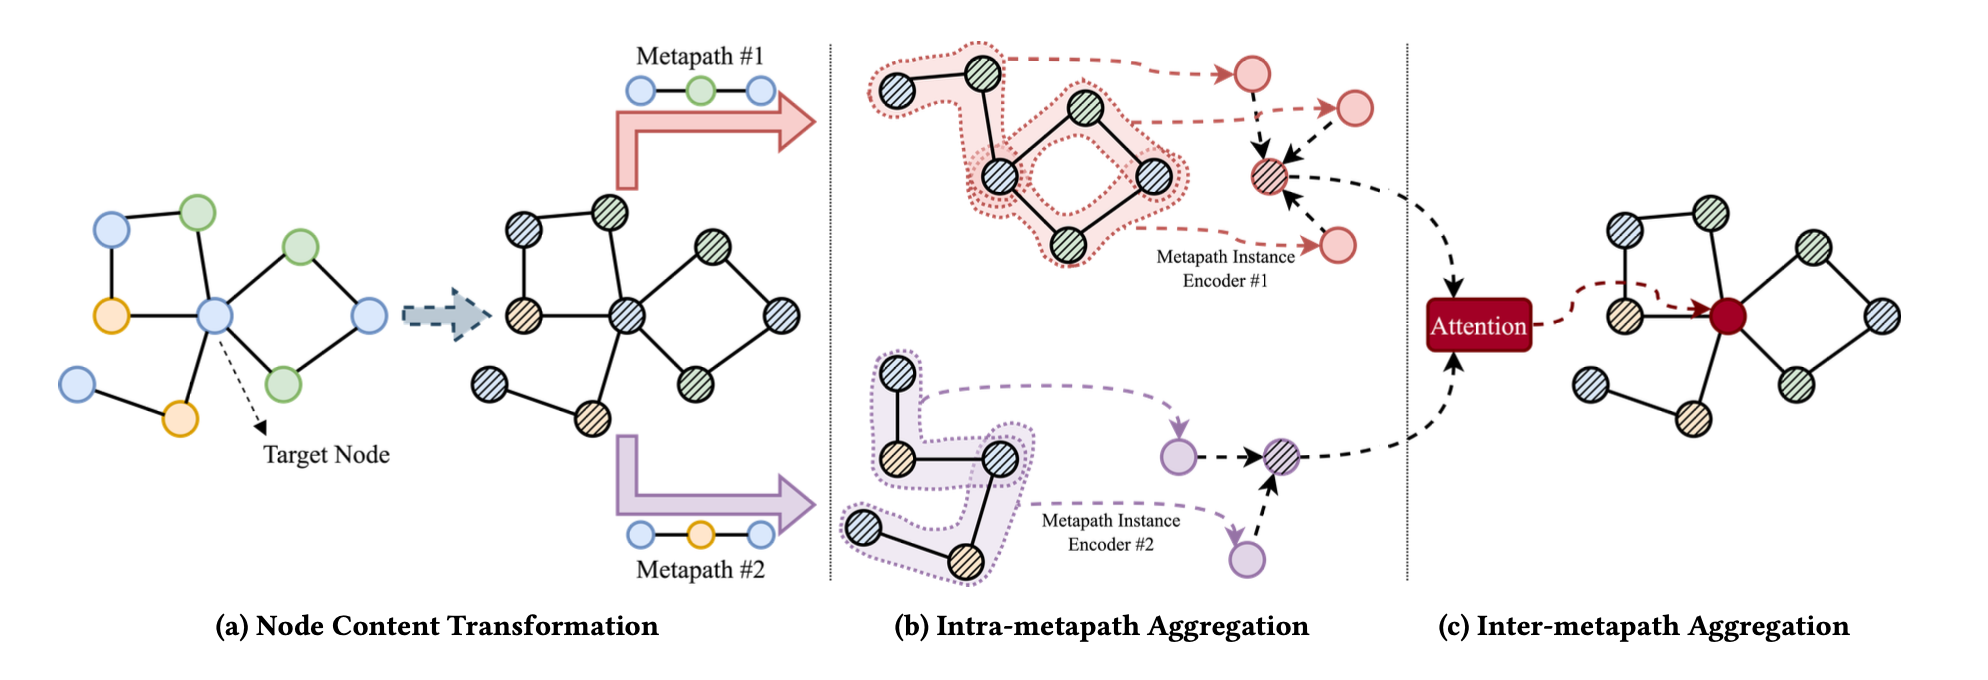
\includegraphics[width=\textwidth]{figs/fig2.png}
  \caption{Kiến trúc tổng thể của MAGNN}
\end{figure*}

\subsection{Tổng hợp intra-metapath}
Cho một metapath $P$, lớp tổng hợp intra-metapath học thông tin cấu trúc và ngữ nghĩa được nhúng trong nút mục tiêu, các lân cận dựa trên metapath và ngữ cảnh ở giữa bằng cách mã hóa cấu hình metapath của $P$. Gọi $P(\nu, u)$ là một cấu hình metapath kết nối nút mục tiêu $\nu$ và lân cận dựa trên metapath $u \in \pmb{\mathcal{N}}^P_{\nu}$, tác giả định nghĩa thêm  nút trung gian của $P(\nu, u)$ như sau $\{ m^{P(\nu, u)} \} = P(\nu, u) \backslash \{ \nu, u \}$. Tổng hợp intra-metapath sử dụng một bộ mã hóa cấu hình metapath để biến đổi tất cả các đặc trưng nút dọc theo một cấu hình metapath thành một vector duy nhất,
\begin{equation}
  \mathbf{h}_{P(\nu, u)} = f_{\theta} (P(\nu, u)) = f_{\theta} \left( \mathbf{h'}_{\nu}, \mathbf{h'}_{u}, \{ \mathbf{h'}_{t}, \forall t \in \{m^{P(\nu, u)}\} \} \right)
\end{equation}
trong đó, $\mathbf{h}_{P(\nu, u)} \in \mathbb{R}^{d'}$ có số chiều là $d'$. Để đơn giản, ta dùng $P(\nu, u)$ để biểu diễn một cấu hình đơn, mặc dù có thể có nhiều cấu hình kết nối 2 nút. Phần sau sẽ giới thiệu một vài lựa chọn của bộ mã hóa cấu hình metapath tốt.

Sau khi mã hóa các cấu hình metapath thành biểu diễn vector, tác giả áp dụng một lớp chú ý đồ thị [28] để  tính tổng trọng số các cấu hình metapath của $P$ liên quan đến nút đích $\nu$. Ý tưởng chính là các cấu hình metapath khác nhau sẽ đóng góp vào biểu diễn nút mục tiêu với mức độ khác nhau. Chúng ta có thể mô hình hóa điều này bằng cách học một trọng số chuẩn hóa quan trọng $\alpha^P_{\nu u}$ cho mỗi cấu hình metapath và sau đó tính tổng trọng số của tất cả các cấu hình:
\begin{equation}
  \begin{split}
    e^P_{\nu u} &= \text{LeakyReLU} (a^T_P \cdot [\mathbf{h'}_{\nu}\parallel \mathbf{h}_{P(\nu, u)}]), \\
  \alpha ^P_{\nu u} &= \frac{\text{exp}{e^P_{\nu u}}}{\sum _{s \in \pmb{\mathcal{N}}^P_{\nu}} \text{exp} (e^P_{\nu u})}, \\
  \mathbf{h}^P_{\nu} &= \sigma \left( \sum_{u \in \pmb{\mathcal{N}}^P_{\nu}} \alpha ^P_{\nu u} \cdot \mathbf{h}_{P(\nu, u)} \right).
  \end{split}
\end{equation}
Trong đó, $a_P \in \mathbb{R}^{2d'}$ là vector chú ý được tham số hóa cho metapath $P$ và $\parallel$ kí hiệu cho toán tử nối vector. $e^P_{\nu u}$ chỉ độ quan trọng của cấu hình metapath $P(\nu, u)$ đến nút $\nu$, nút sau đó được chuẩn hóa theo các lựa chọn $u \in \pmb{\mathcal{N}}^P_{\nu}$ sử dụng hàm softmax. Do trọng số chuẩn hóa $\alpha ^P_{\nu u}$ được lấy cho tất cả $u \in \pmb{\mathcal{N}}^P_{\nu}$, chúng được sử dụng để tính toán một tổ hợp có trọng số của các biểu diễn của các cấu hình metapath cho nút $\nu$. Cuối cùng, đầu ra chạy qua hàm kích hoạt $\sigma (\cdot)$.

Cơ chế chú ý cũng có thể được mở rộng thành nhiều nhánh, điều giúp ổn định quá trình học và giảm đi phương sai lớn từ tính không đồng nhất của đồ thị. Nghĩa là, chúng ta thực hiện $K$ cơ chế chú ý độc lập và sau đó nối đầu ra của chúng lại, kết quả thu được trong biểu thức sau:
\begin{equation}
  \mathbf{h}^P_{\nu} = \parallel ^K_{k=1} \sigma \left( \sum_{u \in \pmb{\mathcal{N}}^P_{\nu}} \left[ \alpha ^P_{\nu u} \right]_k \cdot \mathbf{h}_{P(\nu, u)} \right)
\end{equation} 
trong đó $\left[ \alpha ^P_{\nu u} \right]_k$ là trọng số chuẩn hóa của cấu hình metapath $P(\nu, u)$ đến nút $\nu$ tại nhánh chú ý thứ $k$.

Tóm lại, với các vector đặc trưng $\mathbf{h'}_{u} \in \mathbb{R}^{d'} \forall u \in \pmb{\mathcal{V}}$ và tập các metapaths $\pmb{\mathcal{P}}_A = {P_1, P_2, ..., P_M}$ bắt đầu hoặc kết thúc với loại nút $A \in \pmb{\mathcal{A}}$, tổng hợp của MAGNN sinh $M$ biểu diễn metapath-specific vector của nút đích $\nu \in \pmb{\mathcal{V}}_A$, kí hiệu là $\{ \mathbf{h}^{P_1}_{\nu}, \mathbf{h}^{P_2}_{\nu}, ... , \mathbf{h}^{P_M}_{\nu} \}$. Mỗi $\mathbf{h}^{P_1}_{\nu} \in \mathbb{R}^{d'}$ (giả sử $K=1$) có thể hiểu là tổng hợp của các cấu hình $P_i-\text{metapath}$ của nút $\nu$, thể hiện một khía cạnh của thông tin chứ chong nút $\nu$.

\subsection{Tổng hợp inter-metapath}
Sau khi tổng hợp dữ liệu nút và cạnh với mỗi metapath, chúng ta cần kết hợp thông tin của tất cả các metapath sử dụng một lớp tổng hợp inter-metapath. Bây giờ với một loại nút $A$, ta có $|\pmb{\mathcal{V}}_A|$ tập các latent vectors: $\{ \mathbf{h}^{P_1}_{\nu}, \mathbf{h}^{P_2}_{\nu}, ... , \mathbf{h}^{P_M}_{\nu} \}$ với $\nu \in \pmb{\mathcal{V}}_A$, với $M$ là số metapaths cho loại $A$. Một các tiếp cận tổng hợp inter-metapath trực tiếp là lấy trung bình element-wise của các vectors nút này. Ta mở rộng cách tiếp cận này bằng cách khai thác cơ chế chú ý để gán các trọng số khác nhau cho các metapaths khác nhau. Phép toán này là có lý vì các metapaths có đóng góp không giống nhau trong một đồ thị không đồng nhất.

Đầu tiên, ta cộng mỗi metapath $P_i \in \pmb{\mathcal{P}}_A$ bằng trung bình các vectors nút metapath-specific đã được biến đổi cho tất cả các nút $\nu \in \pmb{\mathcal{V}}_A$,
\begin{equation}
  \mathbf{s}_{P_i} = \frac{1}{|\pmb{\mathcal{V}}_A|} \sum_{\nu \in \pmb{\mathcal{V}}_A} \text{tanh} \left( \mathbf{M}_A \cdot \mathbf{h}^{P_i}_{\nu} + \mathbf{b}_A \right)
\end{equation}
trong đó, $\mathbf{M}_A \in \mathbb{R}^{d_m \times d'}$ và $\mathbf{b}_A \in \mathbb{R}^{d_m}$ là các tham số học.

Sau đó ta sử dụng cơ chế chú ý để  hợp nhất các vectors nút metapath-specific của $\nu$ như sau:
\begin{equation}
  \begin{split}
    e_{P_i} &= \mathbf{q}^T_A \cdot \mathbf{s}_{P_i}, \\
    \beta _{P_i} &= \frac{\text{exp}(e_{P_i})}{\sum_{P \in \pmb{\mathcal{P}}_A} \text{exp}(e_{P})}, \\
    \mathbf{h}^{\pmb{\mathcal{P}}_A}_{\nu} &= \sum_{P \in \pmb{\mathcal{P}}_A} \beta _{P} \cdot \mathbf{h}^P_{\nu}
  \end{split}
\end{equation}
trong đó, $\mathbf{q}_A \in \mathbb{R}^{d_m}$ laf vector chú ý tham số hóa cho loại nút $A$. $\beta _{P_i}$ có thể hiểu là độ đóng góp tương đối của metapath $P_i$ cho các nút loại $A$. Do $\beta _{P_i}$ được tính toán cho mỗi $P_i \in \pmb{\mathcal{P}}_A$, ta có thể tính tổng có trọng số tất cả các vectors nút metapath-specific của $\nu$.

Cuối cùng, MAGNN sử dụng một biến đổi tuyến tính bổ sung với một hàm phi tuyến để chiếu các nút nhúng vào không gian vector với số chiều đầu ra mong muốn:
\begin{equation}
  \mathbf{h}_{\nu} = \sigma \left( \mathbf{W}_0 \cdot \mathbf{h}^{\pmb{\mathcal{P}}_A}_{\nu} \right)
\end{equation}
trong đó, $\sigma (\cdot)$ là một hàm kích hoạt và $\mathbf{W}_0 \in \mathbb{R}^{d_0 \times d'}$ là một ma trận trọng số. Phép chiếu này là một tác vụ cụ thể. Nó có thể hiểu là một phân loại tuyến tính cho phân loại nút hoặc được coi là hình chiếu vào không gian với các độ đo sự tương tự của nút cho dự đoán liên kết. 

\subsection{Biểu diễn (mã hóa) cấu hình metapath}
Để mã hóa cấu hình metapath trong phần IV.B, ta xem xét ba hàm mã hóa khả dĩ sau: 

\begin{itemize}
  \item Mã hóa trung bình. Hàm này tính toán trung bình theo từng thành phần (element-wise) của nút dọc theo cấu hình metapath $P(v, u)$ :
\end{itemize}
\begin{equation}
  \mathbf{h}_{P(v, u)}=\operatorname{MEAN}\left(\left\{\mathbf{h}_{t}^{\prime}, \forall t \in P(v, u)\right\}\right).
\end{equation}

\begin{itemize}
  \item Mã hóa tuyến tính. Hàm này là một phiên bản mở rộng của mã hóa trung bình, trong đó việc mã hóa được thực hiện dựa trên các biến đổi tuyến tính:
\end{itemize}
\begin{equation}
    \mathbf{h}_{P(v, u)}=\mathbf{W}_{P} \cdot \operatorname{MEAN}\left(\left\{\mathbf{h}_{t}^{\prime}, \forall t \in P(v, u)\right\}\right).
\end{equation}

\begin{itemize}
  \item Mã hóa dựa trên phép quay có quan hệ. Ta xem xét mã hóa một cấu hình metapath dựa trên phép quay có quan hệ trong không gian phức, một phương pháp được đề xuất bởi RotatE [24] để biểu diễn đồ thị tri thức. Hàm mã hóa trung bình và tuyến tính được giới thiệu ở trên coi các cấu hình metapath như một tập hợp, và vì thế chúng bỏ qua thông tin được biểu diễn trong kiến trúc chuỗi của metapath. Trong khi đó, phép quay có quan hệ lại cho phép ta mô hình hóa kiểu tri thức đó. Biết $P(v, u)=\left(t_{0}, t_{1}, \ldots, t_{n}\right)$ with $t_{0}=u$ và $t_{n}=v$, let $R_{i}$ là mối quan hệ giữa nút  $t_{i-1}$ và nút $t_{i}$, gọi $\mathbf{r}_{i}$ là vector mối quan hệ của $R_{i}$, khi đó mã hóa dựa trên phép quay có quan hệ được thể hiện bởi công thức.
\end{itemize}
\begin{equation}
    \begin{aligned}
    & \mathbf{o}_{0}=\mathbf{h}_{t_{0}}^{\prime}=\mathbf{h}_{u}^{\prime}, \\
    & \mathbf{o}_{i}=\mathbf{h}_{t_{i}}^{\prime}+\mathbf{o}_{i-1} \odot \mathbf{r}_{i}, \\
    & \mathbf{h}_{P(v, u)}=\frac{\mathbf{o}_{n}}{n+1},
    \end{aligned}
\end{equation}
trong đó  $\mathbf{h}_{t_{i}}^{\prime}$ và $\mathbf{r}_{i}$ đều là các vector phức, $\odot$ là tích vô hướng. Ta có thể dễ giàng phân tích một vector thực có số chiều là $d^{\prime}$ thành một vector phức có số chiều là $d^{\prime} / 2$ bằng cách coi nửa đầu tiên của vector là phần thực và nửa sau là phần ảo.

\subsection{Huấn luyện mô hình}
Sau khi thực hiện các biến đổi thành phần đã giới thiệu ở các phần trước, ta sẽ thu được biểu diễn cuối cùng của các nút để phục vụ cho các bài toán khác tiếp theo. Tùy theo đặc điểm khác nhau của các bài toán và việc nhãn của các nút có sẵn hay không mà chúng ta có thể huấn luyện mô hình MAGNN theo 2 mô hình (paradigm) chính là học bán giám sát (semi-supervised learning) và học không giám sát (unsupervised learning).

Đối với trường hợp học bán giám sát, với thông tin có được từ một phần nhỏ các nút được gán nhãn, ta có thể học các tham số của mô hình để tối thiểu hóa hàm cross-entropy bằng phương pháp lan truyền ngược (backpropagation) hoặc gradient descent. Và từ đó học được cách biểu diễn nút cho đồ thị không đồng nhất sao cho bảo toàn được nhiều thông tin quan trọng nhất có thể. Hàm tổn thất cross-entropy cho trường hợp học bán giám sát được cho bởi công thức sau:
\begin{equation}
    \mathcal{L}=-\sum_{v \in \mathcal{V}_{L}} \sum_{c=1}^{C} \mathbf{y}_{v}[c] \cdot \log \mathbf{h}_{v}[c]
\end{equation}
trong đó $V_{L}$ là tập hợp các nút có nhãn, $C$ là số lượng phân lớp, $\mathbf{y}_{v}$ là vector one-hot thể hiện nhãn của nút $v$, và $\mathbf{h}_{v}$ là vector xác suất dự báo của nút $v$.

Đối với trường hợp học không giám sát thì ta không có bất kì nhãn của nút nào cả, khi đó ta có thể học các tham số của mô hình bằng cách tối thiểu hóa hàm tổn thất sau đây [20]:
\begin{equation}
    \mathcal{L}=-\sum_{(u, v) \in \Omega} \log \sigma\left(\mathbf{h}_{u}^{\top} \cdot \mathbf{h}_{v}\right)-\sum_{\left(u^{\prime}, v^{\prime}\right) \in \Omega^{-}} \log \sigma\left(-\mathbf{h}_{u^{\prime}}^{\top} \cdot \mathbf{h}_{v^{\prime}}\right),
\end{equation}
trong đó $\sigma(\cdot)$ là hàm sigmoid, $\Omega$ là tập hợp các cặp nút quan sát được (dương tính), $\Omega^{-}$ là tập hợp các cặp nút âm tính được lấy mẫu từ tất cả các cặp nút không quan sát được (phần bù của $\Omega$).

\begin{figure}
  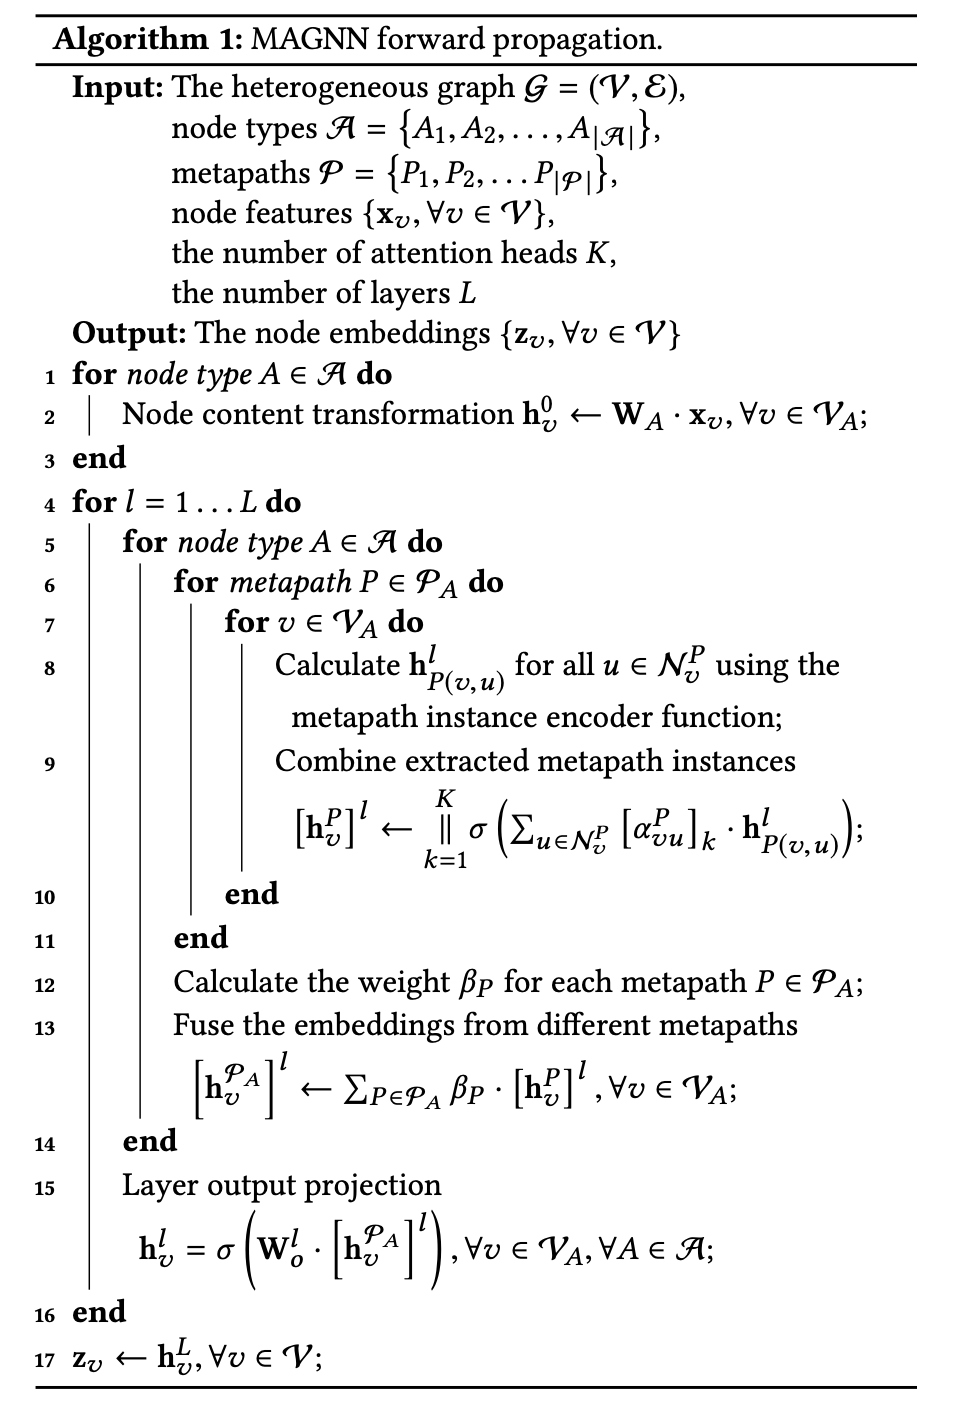
\includegraphics[width=\columnwidth]{figs/alg1.png}
\end{figure}


\section{Ease of Use}

\subsection{Maintaining the Integrity of the Specifications}

The IEEEtran class file is used to format your paper and style the text. All margins, 
column widths, line spaces, and text fonts are prescribed; please do not 
alter them. You may note peculiarities. For example, the head margin
measures proportionately more than is customary. This measurement 
and others are deliberate, using specifications that anticipate your paper 
as one part of the entire proceedings, and not as an independent document. 
Please do not revise any of the current designations.

\section{Prepare Your Paper Before Styling}
Before you begin to format your paper, first write and save the content as a 
separate text file. Complete all content and organizational editing before 
formatting. Please note sections \ref{AA}--\ref{SCM} below for more information on 
proofreading, spelling and grammar.

Keep your text and graphic files separate until after the text has been 
formatted and styled. Do not number text heads---{\LaTeX} will do that 
for you.

\subsection{Abbreviations and Acronyms}\label{AA}
Define abbreviations and acronyms the first time they are used in the text, 
even after they have been defined in the abstract. Abbreviations such as 
IEEE, SI, MKS, CGS, ac, dc, and rms do not have to be defined. Do not use 
abbreviations in the title or heads unless they are unavoidable.

\subsection{Units}
\begin{itemize}
\item Use either SI (MKS) or CGS as primary units. (SI units are encouraged.) English units may be used as secondary units (in parentheses). An exception would be the use of English units as identifiers in trade, such as ``3.5-inch disk drive''.
\item Avoid combining SI and CGS units, such as current in amperes and magnetic field in oersteds. This often leads to confusion because equations do not balance dimensionally. If you must use mixed units, clearly state the units for each quantity that you use in an equation.
\item Do not mix complete spellings and abbreviations of units: ``Wb/m\textsuperscript{2}'' or ``webers per square meter'', not ``webers/m\textsuperscript{2}''. Spell out units when they appear in text: ``. . . a few henries'', not ``. . . a few H''.
\item Use a zero before decimal points: ``0.25'', not ``.25''. Use ``cm\textsuperscript{3}'', not ``cc''.)
\end{itemize}

\subsection{Equations}
Number equations consecutively. To make your 
equations more compact, you may use the solidus (~/~), the exp function, or 
appropriate exponents. Italicize Roman symbols for quantities and variables, 
but not Greek symbols. Use a long dash rather than a hyphen for a minus 
sign. Punctuate equations with commas or periods when they are part of a 
sentence, as in:
\begin{equation}
a+b=\gamma\label{eq}
\end{equation}

Be sure that the 
symbols in your equation have been defined before or immediately following 
the equation. Use ``\eqref{eq}'', not ``Eq.~\eqref{eq}'' or ``equation \eqref{eq}'', except at 
the beginning of a sentence: ``Equation \eqref{eq} is . . .''

\subsection{\LaTeX-Specific Advice}

Please use ``soft'' (e.g., \verb|\eqref{Eq}|) cross references instead
of ``hard'' references (e.g., \verb|(1)|). That will make it possible
to combine sections, add equations, or change the order of figures or
citations without having to go through the file line by line.

Please don't use the \verb|{eqnarray}| equation environment. Use
\verb|{align}| or \verb|{IEEEeqnarray}| instead. The \verb|{eqnarray}|
environment leaves unsightly spaces around relation symbols.

Please note that the \verb|{subequations}| environment in {\LaTeX}
will increment the main equation counter even when there are no
equation numbers displayed. If you forget that, you might write an
article in which the equation numbers skip from (17) to (20), causing
the copy editors to wonder if you've discovered a new method of
counting.

{\BibTeX} does not work by magic. It doesn't get the bibliographic
data from thin air but from .bib files. If you use {\BibTeX} to produce a
bibliography you must send the .bib files. 

{\LaTeX} can't read your mind. If you assign the same label to a
subsubsection and a table, you might find that Table I has been cross
referenced as Table IV-B3. 

{\LaTeX} does not have precognitive abilities. If you put a
\verb|\label| command before the command that updates the counter it's
supposed to be using, the label will pick up the last counter to be
cross referenced instead. In particular, a \verb|\label| command
should not go before the caption of a figure or a table.

Do not use \verb|\nonumber| inside the \verb|{array}| environment. It
will not stop equation numbers inside \verb|{array}| (there won't be
any anyway) and it might stop a wanted equation number in the
surrounding equation.

\subsection{Some Common Mistakes}\label{SCM}
\begin{itemize}
\item The word ``data'' is plural, not singular.
\item The subscript for the permeability of vacuum $\mu_{0}$, and other common scientific constants, is zero with subscript formatting, not a lowercase letter ``o''.
\item In American English, commas, semicolons, periods, question and exclamation marks are located within quotation marks only when a complete thought or name is cited, such as a title or full quotation. When quotation marks are used, instead of a bold or italic typeface, to highlight a word or phrase, punctuation should appear outside of the quotation marks. A parenthetical phrase or statement at the end of a sentence is punctuated outside of the closing parenthesis (like this). (A parenthetical sentence is punctuated within the parentheses.)
\item A graph within a graph is an ``inset'', not an ``insert''. The word alternatively is preferred to the word ``alternately'' (unless you really mean something that alternates).
\item Do not use the word ``essentially'' to mean ``approximately'' or ``effectively''.
\item In your paper title, if the words ``that uses'' can accurately replace the word ``using'', capitalize the ``u''; if not, keep using lower-cased.
\item Be aware of the different meanings of the homophones ``affect'' and ``effect'', ``complement'' and ``compliment'', ``discreet'' and ``discrete'', ``principal'' and ``principle''.
\item Do not confuse ``imply'' and ``infer''.
\item The prefix ``non'' is not a word; it should be joined to the word it modifies, usually without a hyphen.
\item There is no period after the ``et'' in the Latin abbreviation ``et al.''.
\item The abbreviation ``i.e.'' means ``that is'', and the abbreviation ``e.g.'' means ``for example''.
\end{itemize}
An excellent style manual for science writers is \cite{b7}.

\subsection{Authors and Affiliations}
\textbf{The class file is designed for, but not limited to, six authors.} A 
minimum of one author is required for all conference articles. Author names 
should be listed starting from left to right and then moving down to the 
next line. This is the author sequence that will be used in future citations 
and by indexing services. Names should not be listed in columns nor group by 
affiliation. Please keep your affiliations as succinct as possible (for 
example, do not differentiate among departments of the same organization).

\subsection{Identify the Headings}
Headings, or heads, are organizational devices that guide the reader through 
your paper. There are two types: component heads and text heads.

Component heads identify the different components of your paper and are not 
topically subordinate to each other. Examples include Acknowledgments and 
References and, for these, the correct style to use is ``Heading 5''. Use 
``figure caption'' for your Figure captions, and ``table head'' for your 
table title. Run-in heads, such as ``Abstract'', will require you to apply a 
style (in this case, italic) in addition to the style provided by the drop 
down menu to differentiate the head from the text.

Text heads organize the topics on a relational, hierarchical basis. For 
example, the paper title is the primary text head because all subsequent 
material relates and elaborates on this one topic. If there are two or more 
sub-topics, the next level head (uppercase Roman numerals) should be used 
and, conversely, if there are not at least two sub-topics, then no subheads 
should be introduced.

\subsection{Figures and Tables}
\paragraph{Positioning Figures and Tables} Place figures and tables at the top and 
bottom of columns. Avoid placing them in the middle of columns. Large 
figures and tables may span across both columns. Figure captions should be 
below the figures; table heads should appear above the tables. Insert 
figures and tables after they are cited in the text. Use the abbreviation 
``Fig.~\ref{fig}'', even at the beginning of a sentence.

\begin{table}[htbp]
\caption{Table Type Styles}
\begin{center}
\begin{tabular}{|c|c|c|c|}
\hline
\textbf{Table}&\multicolumn{3}{|c|}{\textbf{Table Column Head}} \\
\cline{2-4} 
\textbf{Head} & \textbf{\textit{Table column subhead}}& \textbf{\textit{Subhead}}& \textbf{\textit{Subhead}} \\
\hline
copy& More table copy$^{\mathrm{a}}$& &  \\
\hline
\multicolumn{4}{l}{$^{\mathrm{a}}$Sample of a Table footnote.}
\end{tabular}
\label{tab1}
\end{center}
\end{table}

\begin{figure}[htbp]
\centerline{
\includegraphics{fig1.png}}
\caption{Example of a figure caption.}
\label{fig}
\end{figure}

Figure Labels: Use 8 point Times New Roman for Figure labels. Use words 
rather than symbols or abbreviations when writing Figure axis labels to 
avoid confusing the reader. As an example, write the quantity 
``Magnetization'', or ``Magnetization, M'', not just ``M''. If including 
units in the label, present them within parentheses. Do not label axes only 
with units. In the example, write ``Magnetization (A/m)'' or ``Magnetization 
\{A[m(1)]\}'', not just ``A/m''. Do not label axes with a ratio of 
quantities and units. For example, write ``Temperature (K)'', not 
``Temperature/K''.

\section*{Acknowledgment}

The preferred spelling of the word ``acknowledgment'' in America is without 
an ``e'' after the ``g''. Avoid the stilted expression ``one of us (R. B. 
G.) thanks $\ldots$''. Instead, try ``R. B. G. thanks$\ldots$''. Put sponsor 
acknowledgments in the unnumbered footnote on the first page.

\section*{References}

Please number citations consecutively within brackets \cite{b1}. The 
sentence punctuation follows the bracket \cite{b2}. Refer simply to the reference 
number, as in \cite{b3}---do not use ``Ref. \cite{b3}'' or ``reference \cite{b3}'' except at 
the beginning of a sentence: ``Reference \cite{b3} was the first $\ldots$''

Number footnotes separately in superscripts. Place the actual footnote at 
the bottom of the column in which it was cited. Do not put footnotes in the 
abstract or reference list. Use letters for table footnotes.

Unless there are six authors or more give all authors' names; do not use 
``et al.''. Papers that have not been published, even if they have been 
submitted for publication, should be cited as ``unpublished'' \cite{b4}. Papers 
that have been accepted for publication should be cited as ``in press'' \cite{b5}. 
Capitalize only the first word in a paper title, except for proper nouns and 
element symbols.

For papers published in translation journals, please give the English 
citation first, followed by the original foreign-language citation \cite{b6}.

\begin{thebibliography}{00}
\bibitem{b1} G. Eason, B. Noble, and I. N. Sneddon, ``On certain integrals of Lipschitz-Hankel type involving products of Bessel functions,'' Phil. Trans. Roy. Soc. London, vol. A247, pp. 529--551, April 1955.
\bibitem{b2} J. Clerk Maxwell, A Treatise on Electricity and Magnetism, 3rd ed., vol. 2. Oxford: Clarendon, 1892, pp.68--73.
\bibitem{b3} I. S. Jacobs and C. P. Bean, ``Fine particles, thin films and exchange anisotropy,'' in Magnetism, vol. III, G. T. Rado and H. Suhl, Eds. New York: Academic, 1963, pp. 271--350.
\bibitem{b4} K. Elissa, ``Title of paper if known,'' unpublished.
\bibitem{b5} R. Nicole, ``Title of paper with only first word capitalized,'' J. Name Stand. Abbrev., in press.
\bibitem{b6} Y. Yorozu, M. Hirano, K. Oka, and Y. Tagawa, ``Electron spectroscopy studies on magneto-optical media and plastic substrate interface,'' IEEE Transl. J. Magn. Japan, vol. 2, pp. 740--741, August 1987 [Digests 9th Annual Conf. Magnetics Japan, p. 301, 1982].
\bibitem{b7} M. Young, The Technical Writer's Handbook. Mill Valley, CA: University Science, 1989.
\end{thebibliography}
\vspace{12pt}
\color{red}
IEEE conference templates contain guidance text for composing and formatting conference papers. Please ensure that all template text is removed from your conference paper prior to submission to the conference. Failure to remove the template text from your paper may result in your paper not being published.

\end{document}
